\section{Experiments and Discussion}
\label{sec:experiments}

Our framework allows us to define a PGM once and compile it into task-specific flows; we evaluate both compiled regimes---\textit{Causal Alignment} for mechanistic queries and \textit{Inference Alignment} for statistical queries---asking whether structure-aligned flows support all three levels of Pearl's causal hierarchy, whether the compiled inference engines provide accurate amortized inference, and how static and dynamic conditioning compare. We compare four methods: \textbf{CAREFL} \citep{khemakhem2021causal}, an affine autoregressive flow baseline; \textbf{Guided}, an unstructured flow trained on the joint and conditioned via reconstruction guidance; and our structure-aligned flows with \textbf{Static} (condition on $x_1$) and \textbf{Dynamic} (condition on $x_t$) conditioning.

\subsection{Experimental Setup}

We train and evaluate on synthetic $4$-node nonlinear PGMs with randomly generated structural equations, giving each model access to samples from the joint distribution (see Appendix~\ref{app:experiments} for details). Graph sizes are bounded by evaluation, not training: the number of supported queries grows rapidly with graph size and every inference-direction query requires its own NUTS ground-truth reference, so we evaluate exhaustively at $n{=}4$ and $n{=}8$ rather than sparsely at larger $n$.

We report the Sliced Wasserstein Distance (SWD) as our primary metric, since the nonlinear PGMs do not admit tractable density evaluation for all queries of interest; it is normalized by $\sqrt{N\,D}$ to be comparable across queries of differing dimension and sample size (so absolute magnitudes are small---the meaningful signal is the \emph{relative} ordering between methods). Where ground-truth densities are available (linear-Gaussian PGMs on causal queries), we additionally report the KL divergence (Appendix~\ref{app:kl-linear}), which corroborates the SWD ranking on a calibrated scale for the methods that define a tractable conditional density (guided sampling does not, so it is scored by SWD only).

\paragraph{Reading the plots.} Box plots aggregate PGM and learner seeds \emph{and all supported conditional queries of each graph}; given the seed counts we report observed spread rather than significance tests. The sharpest claims (moralization, sample efficiency) are measured against exact ground-truth posteriors (Appendix~\ref{app:additional-experiments}).

\subsection{Causal Alignment}

For Causal Alignment, we set the structure of the flow to match the structure of the PGM. This alignment enables the flow to support interventional and counterfactual queries.


\begin{figure*}[t]
    \centering
    \begin{subfigure}[t]{0.32\textwidth}
        \centering
        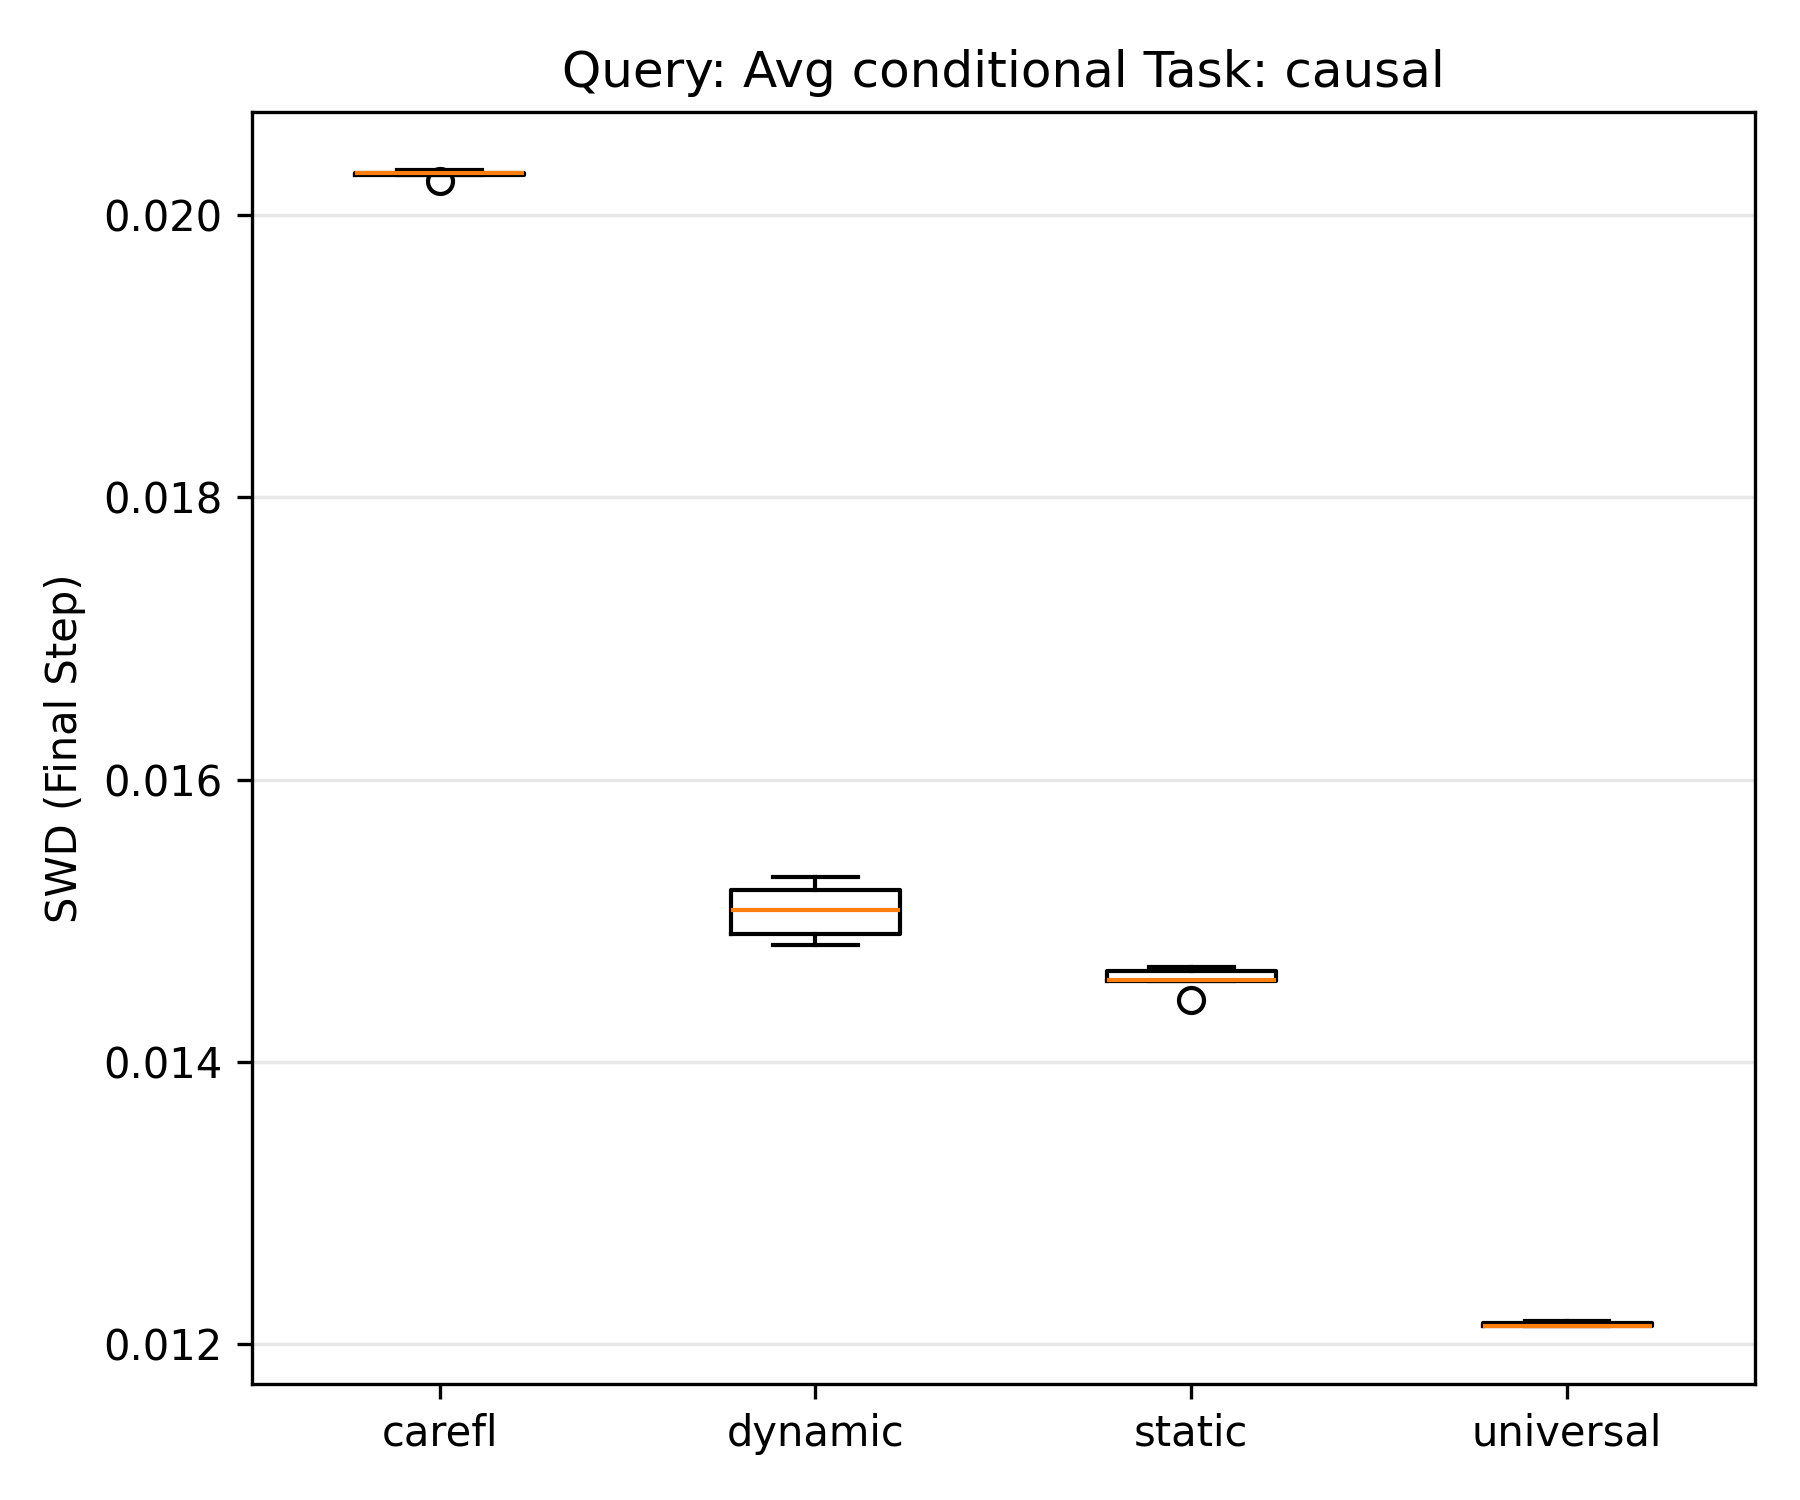
\includegraphics[width=\textwidth]{images/experimental_figures/nonlinear/final_box_swd_pgms_all_task_causal_queries_avg_conditional.png}
        \caption{Interventional $p(y\mid \mathrm{do}(x))$}
        \label{fig:swd-nonlinear-causal}
    \end{subfigure}
    \hfill
    \begin{subfigure}[t]{0.32\textwidth}
        \centering
        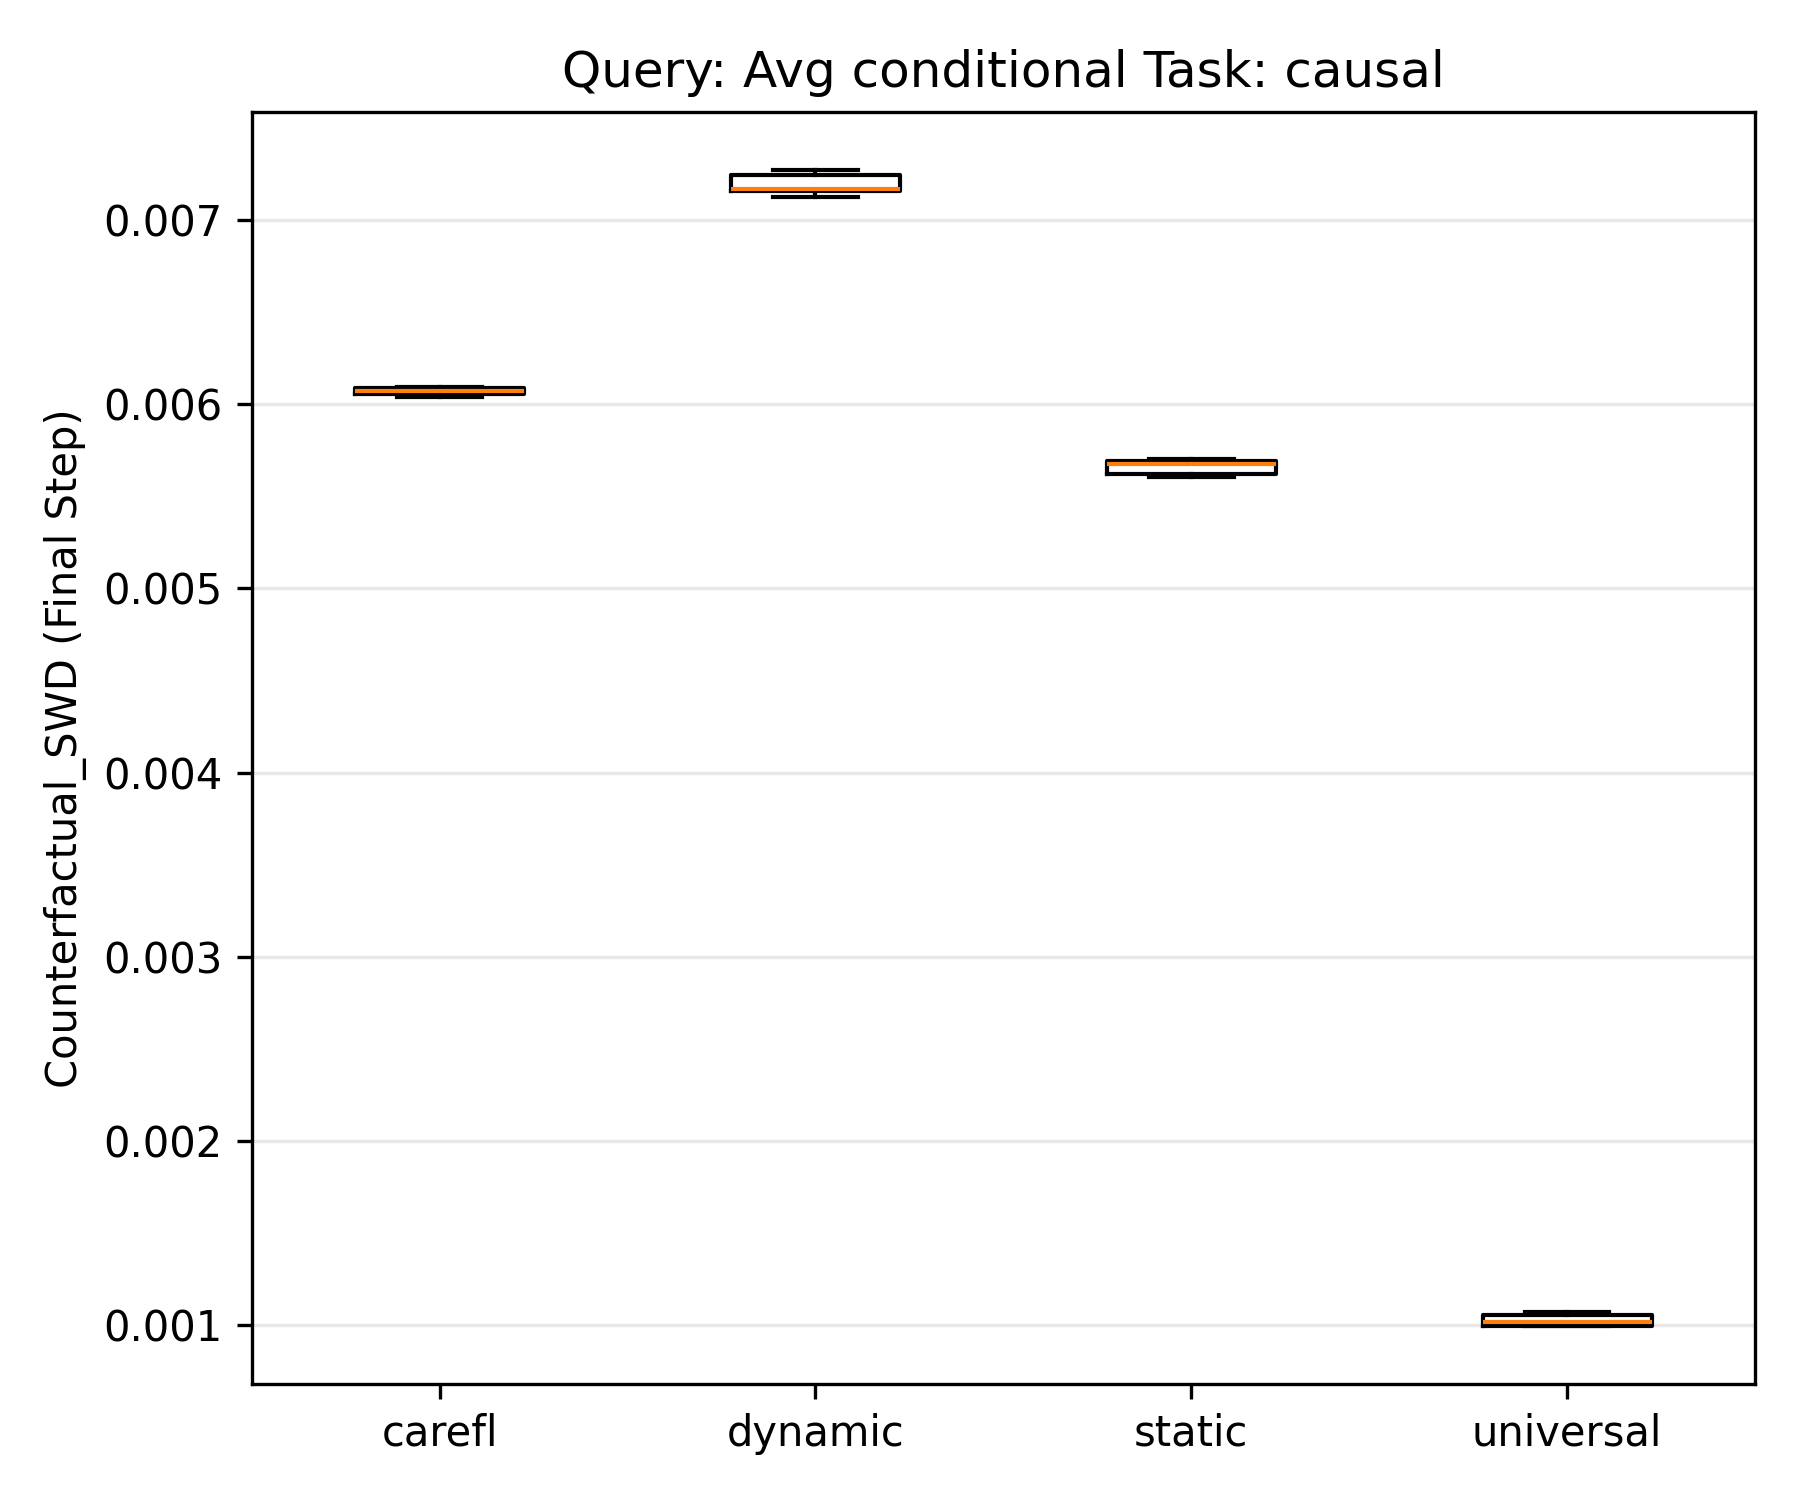
\includegraphics[width=\textwidth]{images/experimental_figures/nonlinear/final_box_counterfactual_swd_pgms_all_task_causal_queries_avg_conditional.png}
        \caption{Counterfactual}
        \label{fig:counterswd-nonlinear-causal}
    \end{subfigure}
    \hfill
    \begin{subfigure}[t]{0.32\textwidth}
        \centering
        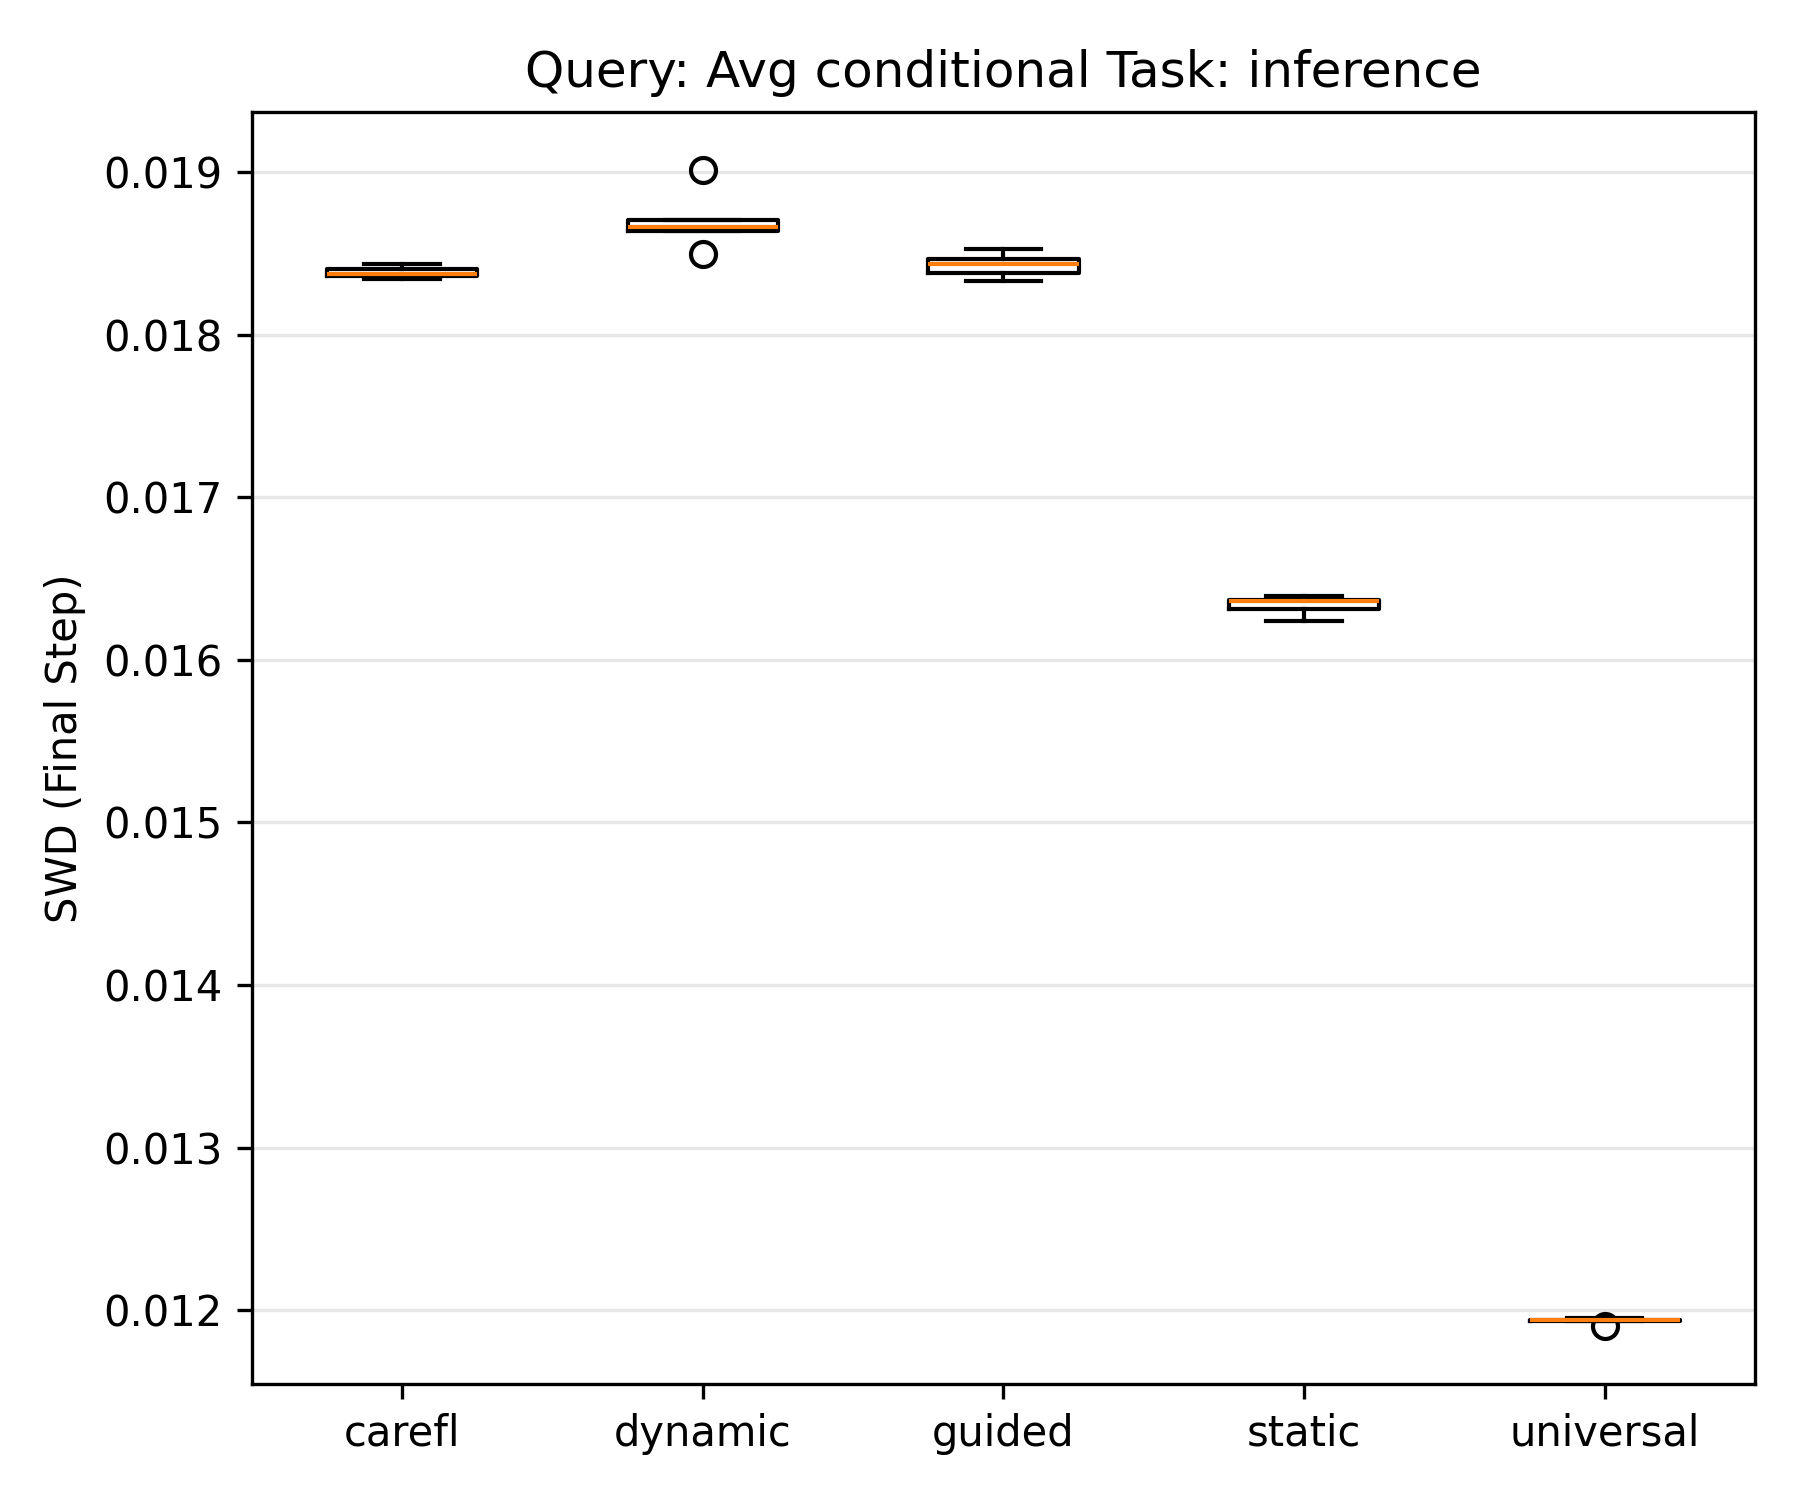
\includegraphics[width=\textwidth]{images/experimental_figures/nonlinear/final_box_swd_pgms_all_task_inference_queries_avg_conditional.png}
        \caption{Inference $p(\mathrm{pa}\mid\mathrm{ch})$}
        \label{fig:inference-nonlinear-pgm}
    \end{subfigure}
    \caption{\textbf{Normalized Sliced Wasserstein Distance on nonlinear 4-node PGMs}, aggregated over the supported conditional queries, 3 PGM seeds and 3 learner seeds. On these nonlinear mechanisms the CNF variants (Static, Dynamic) are competitive with or better than CAREFL on both causal query types (a, b); all methods are comparable on these small, well-sampled inference problems (c). (On the \emph{linear} benchmarks CAREFL's affine class exactly matches the mechanisms and excels, particularly on counterfactuals; Appendix~\ref{app:results}.)}
    \label{fig:pgm-results}
\end{figure*}

\paragraph{Interventional Queries (Level 2).} In the causally aligned flow, an intervention $\mathrm{do}(x)$ is realized by clamping the block of $x$ to the intervened value while integrating all other blocks as usual. The clamped block ignores its own parents, so the flow samples exactly the mutilated graph of the intervention, yielding $p(y \mid \mathrm{do}(x))$. In general this \emph{differs} from the observational conditional $p(y \mid x)$, which additionally updates the distribution of $x$'s ancestors through back-door paths---a task for the inference-aligned model. The two coincide whenever the conditioning set leaves no back-door path to update; two sufficient conditions cover our benchmarks: the conditioning set is \emph{ancestrally closed} (Theorem~\ref{thm:marginalization}; e.g.\ root nodes and topological prefixes), or it contains every direct parent of the target and none of its descendants (both queries then reduce to the same mechanism conditional by the local Markov property). Every causal-mode benchmark query below is of one of these forms.

\paragraph{Counterfactual Queries (Level 3).} Counterfactual queries use the abduction--action--prediction procedure of Section~\ref{sec:counterfactuals}, which requires a bijective correspondence between an observation and the exogenous noise that produced it. Diffusion models with stochastic samplers lack such a correspondence; diffusion-based causal models recover one by replacing the stochastic sampler with a deterministic DDIM or probability-flow-ODE inversion \citep{sanchez2022diffusion, chao2023interventional}---the same flow-inversion principle used here---whereas CNFs provide the bijection natively, alongside exact density evaluation. The two are not equally exact: DDIM inversion carries a first-order abduction bias that a CNF's tolerance-controlled solve does not (Proposition~\ref{prop:abduction-error}; measured in Section~\ref{sec:backbone-ablation}). Recall also that the recovered noise coincides with the \emph{true} exogenous noise only under the conditions of Theorem~\ref{thm:level3}, which cover our synthetic benchmarks (Remark~\ref{rem:cf-identifiability}).

\paragraph{Results.} At the observational level (Level 1), all flow-based methods recover the joint distribution $p(y)$ comparably well, with no consistent separation between structured and unstructured variants (joint-distribution SWD in Appendix Figure~\ref{fig:nonlinear-joint}); we therefore focus the main text on the interventional and counterfactual levels, where structure is load-bearing. Figures~\ref{fig:swd-nonlinear-causal} and~\ref{fig:counterswd-nonlinear-causal} show the comparison on the nonlinear PGMs (per-graph breakdown in Appendix Figure~\ref{fig:swd-linear-v-nonlinear}). On these nonlinear mechanisms, Static and Dynamic match or outperform CAREFL on interventional queries, and all three are close on counterfactuals (Static and CAREFL essentially tied, Dynamic within ${\sim}20\%$). The picture inverts on the \emph{linear} benchmarks (Appendix~\ref{app:results}): there CAREFL's affine transformations coincide exactly with the true mechanism class, and it excels---most visibly on counterfactuals, where abduction through the exactly-matched affine inverse is nearly exact. Both observations are two sides of the same expressivity argument: the affine transformations $x' = s(x_{<i}) \cdot x + t(x_{<i})$ that CAREFL needs for identifiability are not universal density approximators \citep[App.~B--C]{khemakhem2021causal}---exact when the mechanisms are affine, limited when they are not---whereas our CNFs realize any smooth monotone noise-to-value map \citep{zhang2020approximationcapabilitiesneuralodes}. Enforcing causal structure through the \emph{topology} of the vector field rather than the algebraic form of the coupling retains expressivity that affine flows lack.

An ablation replacing each block's velocity field with a per-node denoising diffusion model (the construction of DCM and Diff-SCM) at matched budgets shows the two backbones agree on interventional queries at moderate-to-high NFE while the diffusion variant's abduction error decays only at first order---evidence that the compiled structure, not the choice of continuous-time generative model, is load-bearing (Appendix~\ref{app:additional-experiments}, Section~\ref{sec:backbone-ablation}).

\paragraph{Inference alignment, moralization, and amortization.} Three further results confirm the framework's inference-direction properties and are given in full in Appendix~\ref{app:additional-experiments}: on these small, well-sampled graphs all methods perform amortized posterior inference comparably (Figure~\ref{fig:pgm-results}c); \rev{an ablation on a linear-Gaussian collider shows the compiled co-parent dependency is \emph{necessary}---without it the flow provably cannot represent the induced posterior correlation} (recovered $-0.94$ vs.\ analytic $-0.92$; ablated: $\approx 0$); and the compiled inference engine amortizes, answering posterior queries ${\sim}11\times$ faster than per-query NUTS beyond a crossover of $K^\star \approx 22$ queries.

\subsection{Colored-MNIST: Intervening vs.\ Conditioning \cam{on Images}}
\label{sec:colored-mnist}


\begin{figure}[t]
    \centering
    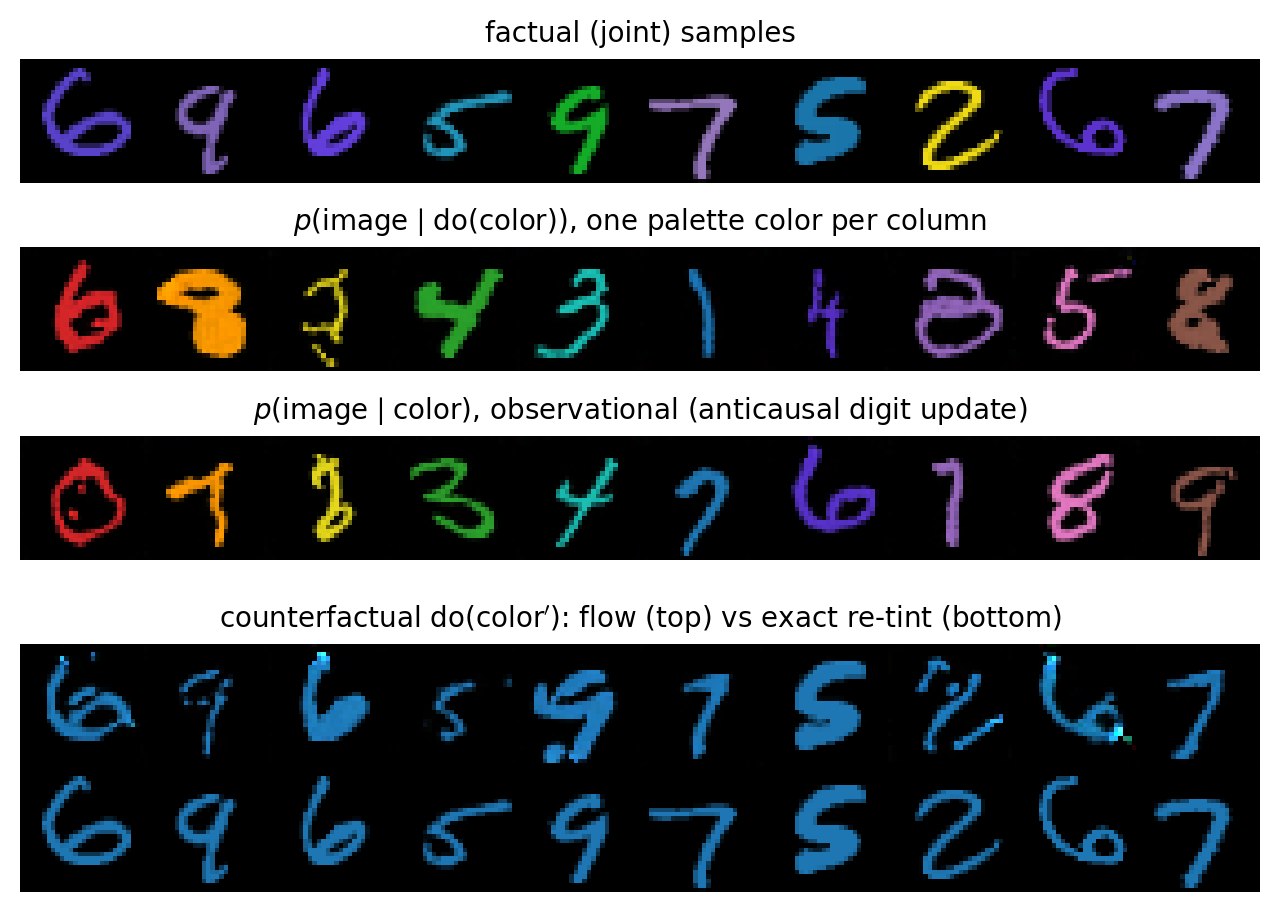
\includegraphics[width=0.44\columnwidth]{images/colored_mnist_conv_strips.png}
    \caption{\textbf{Colored-MNIST samples.} Row 1: factual samples from the joint. Row 2: causal-alignment samples from $p(\mathrm{image} \mid \mathrm{do}(\mathrm{color}{=}\mathrm{palette}_j))$---the forced color does not change which digit appears. Row 3: inference-alignment samples from the observational $p(\mathrm{image} \mid \mathrm{color}{=}\mathrm{palette}_j)$---column $j$ mostly shows its correlated digit $j$. Row 4: counterfactual re-coloring of row 1's factuals under $\mathrm{do}(\mathrm{color}{=}\mathrm{palette}_5)$: the causal flow inverts each image to its exogenous noise and re-generates with the color forced (upper strip); the lower strip is the exact ground truth.}
    \label{fig:colored-mnist-strips}
    \vspace{-1.2\baselineskip}
\end{figure}


The synthetic benchmarks demonstrate non-trivial graph structure at low dimension and MNIST a higher-dimensional problem with trivial structure (Appendix~\ref{app:additional-experiments}); Colored-MNIST combines both, and makes the paper's central distinction---conditioning versus intervening---\emph{visible}. The causal graph is $\text{digit} \to \text{color}$, $(\text{digit}, \text{color}) \to \text{image}$: each digit class has a palette color applied with probability $\rho = 0.8$ (otherwise a uniformly random palette color, plus Gaussian jitter), and the image is the grayscale digit tinted by the color ($28{\times}28{\times}3 = 2352$ dimensions). Because we author this mechanism, the digit posterior $p(d \mid \mathrm{color})$ is available in closed form, and interventional and counterfactual ground truth can be sampled exactly.

From this single specification the compiler produces both artifacts: the causal-alignment model answers $p(\mathrm{image} \mid \mathrm{do}(\mathrm{color}))$ by clamping the color block, while the inference-alignment model (compiled order $[\mathrm{color}, \mathrm{image}, \mathrm{digit}]$) answers the \emph{observational} conditionals, which require the anticausal belief update through $\mathrm{color} \leftarrow \mathrm{digit}$. The block abstraction also gives architectural modularity: any network respecting the block interface (state, parents, time) can serve as a block's velocity field, so we use a small convolutional U-Net for the image block and MLPs for the vector blocks (static conditioning, 8M-parameter budget).

Figure~\ref{fig:colored-mnist-heatmaps} shows the result. Under $\mathrm{do}(\mathrm{color}{=}\mathrm{palette}_j)$ the digit marginal is uniform for every $j$---forcing a color does not change which digit is drawn---and the flow reproduces this. Under \emph{conditioning} on the same color values, the exact posterior concentrates $0.79$ of its mass on the correlated digit, and the flow recovers this diagonal structure ($0.55$--$0.75$ across colors; residual conditional-generation error, not structural---with ground-truth images the flow recovers the exact posterior peak to within $0.02$). The same contrast is visible directly in samples (Figure~\ref{fig:colored-mnist-strips}): under intervention, random digits appear in every color; under conditioning, each color mostly produces its correlated digit. The inference-aligned flow also answers the fully anticausal classification query $p(\mathrm{digit} \mid \mathrm{color}, \mathrm{image})$ with $98.8\%$ held-out accuracy---amortized, with no per-query inference procedure. One honest caveat: at $\rho = 0.8$ the off-palette pairs row 4 produces appear in training with probability ${\sim}2\%$---rare-shot rather than zero-shot. Retraining at $\rho = 1$ removes them entirely and the result is unchanged in kind: interventions extrapolate to every never-seen (digit, color) pair, and counterfactual re-coloring becomes genuinely zero-shot, with residual failures concentrated in abduction (Appendix~\ref{app:colored-mnist-rho1}).

Comparing static and dynamic conditioning on this benchmark (MLP backbone at a matched $8$M budget; mean normalized SWD over $7$--$8$ independently trained runs per mode, seed s.d.\ $\leq 0.3$), both modes answer every compiled query family accurately, with all errors at the $10^{-4}$ scale of the joint-modeling floor. On the joint the two are indistinguishable ($1.7$ vs $1.6 \times 10^{-4}$); on the conditionals dynamic pays a modest relative penalty---$5.3$ vs $1.7 \times 10^{-4}$ on the causal $p(\mathrm{image} \mid \mathrm{digit}, \mathrm{color})$ and $7.8$ vs $1.9 \times 10^{-4}$ on the observational $p(\mathrm{image} \mid \mathrm{color})$, i.e.\ $3$--$4\times$---consistent with the depth-and-informativeness mechanism of Section~\ref{sec:chain-stiffness}.


\subsection{Scaling Dynamic Conditioning: The Price of Parallelism}
\label{sec:chain-stiffness}

The results above leave static and dynamic conditioning competitive, and dynamic additionally samples all blocks in a single parallel ODE solve. Is that parallelism a free win? At sampling time, dynamic conditioning clamps observed conditions to a trajectory integrated backward from the observed value; we stress-test how this scales with the depth of nested dependencies on chains $x_0 \to \cdots \to x_{n-1}$, conditioning on the leaf and inferring the root---the query whose conditioning signal must propagate deepest. Since any stationary chain's root--leaf correlation decays geometrically---deep chains would become easy-to-fake tasks with vanishing headroom over the prior---we use a unit-root random walk, $x_{k+1} = x_k + \sigma\varepsilon_k$ with $\sigma = 0.2$ and $x_0 \sim \mathcal{N}(0,1)$: each link is near-deterministic (conditional s.d.\ $0.2$ against unit-scale marginals) yet the root--leaf correlation $1/\sqrt{1 + (n{-}1)\sigma^2}$ decays only polynomially, still $0.67$ at $n{=}32$. We train both modes at matched parameter budgets for $n \in \{2, 4, 8, 16, 32\}$ and measure the $2$-Wasserstein distance to the exact Gaussian posterior (Figure~\ref{fig:chain-stiffness}).

At a matched solver budget (Figure~\ref{fig:chain-stiffness}, left; equal step counts give the two modes near-equal FLOPs, static's $n$ small-block solves matching dynamic's full-network evaluations), static error grows slowly and monotonically with depth ($0.19$ to $0.52$) as its sequential block solves accumulate error, staying well below the prior baseline throughout. Dynamic starts ${\sim}2.8\times$ worse and \emph{degrades} with depth, until at $n{=}32$ its error ($0.88 \pm 0.14$) exceeds that of ignoring the evidence entirely ($0.65$)---conditioning has become actively harmful. Three diagnostics locate the failure. \emph{First}, static \emph{converges} with solver effort (error flat beyond ${\sim}32$ RK4 steps at every depth), whereas dynamic \emph{anti-converges}---error \emph{increases} with solver accuracy ($0.72$ at $4$ steps to $0.96$ at $128$ for $n{=}32$): faithfully integrating a velocity field evaluated off-distribution amplifies its error, and coarse integration acts as accidental regularization. \emph{Second}, the source: the clamped condition trajectory leaves the training distribution---its $z$-score against the training-interpolant marginal grows from $6.7$ at $n{=}4$ to $86$ at $n{=}32$ under an informative ($90$th-percentile) observation---because deeper evidence is more informative, landing the backward integration off the manifold the network was trained on. \emph{Third}, the naive hypothesis---depth makes the dynamic ODE stiffer---fails instructively: peak velocities do grow with depth ($2.9\times$ the unconditional level at $n{=}2$ to $41\times$ at $n{=}32$) but \emph{only at the clamped condition block}, whose velocity is discarded at every step: a futile corrective response, and a pure OOD diagnostic. The integrated blocks stay at $2$--$4\times$ (static's ${\sim}1\times$)---the learned dynamics never stiffen; the error enters through the conditioning trajectory itself. The same grading appears in the paper's own benchmarks: on the $8$-node linear graphs, dynamic's conditional error relative to static grows with the number of conditioning variables ($3.1\times$ at one to $11.4\times$ at five or more), while static, CAREFL, and the unstructured baselines remain flat. The practical reading: dynamic's parallelism is paid for in error that is \emph{structural}---growing with the depth and informativeness of the evidence, an order of magnitude noisier across seeds, not repairable by solver effort---marking the conditioning trajectory itself as the object to fix (Section~\ref{sec:future_work}); static's error is solver-converged and predictable, responding to the knobs a practitioner controls.

\paragraph{Relation to language-model decoding.} The static/dynamic split mirrors the autoregressive-vs-diffusion divide in language models: static is ancestral sampling in a compiled order; dynamic parallels diffusion-LM decoding, where all positions co-evolve and prompt tokens are clamped during the reverse process. The failure modes translate: parallel decoding's error is likewise mechanism-set---within-step tokens commit independently, and sequence-level correctness needs steps scaling with length \citep{liu2024copula,feng2025theoretical}---and \emph{inaccurate} sampling has flattered masked-diffusion metrics much as coarse integration flatters dynamic \citep{zheng2024masked}. Off-manifold clamping is documented for \emph{continuous}-state diffusion \citep{lugmayr2022repaint,ning2023input}---our chains isolate a stronger form, injected purely through the conditioning trajectory even for a perfect model---while masked \emph{discrete} diffusion escapes it, clamped tokens staying on the training manifold \citep{ou2024absorbing}. Where adaptive token order is decisive for masked diffusion \citep{kim2025train}, our inference alignment chooses it at compile time.

\begin{figure*}[t!]
    \centering
    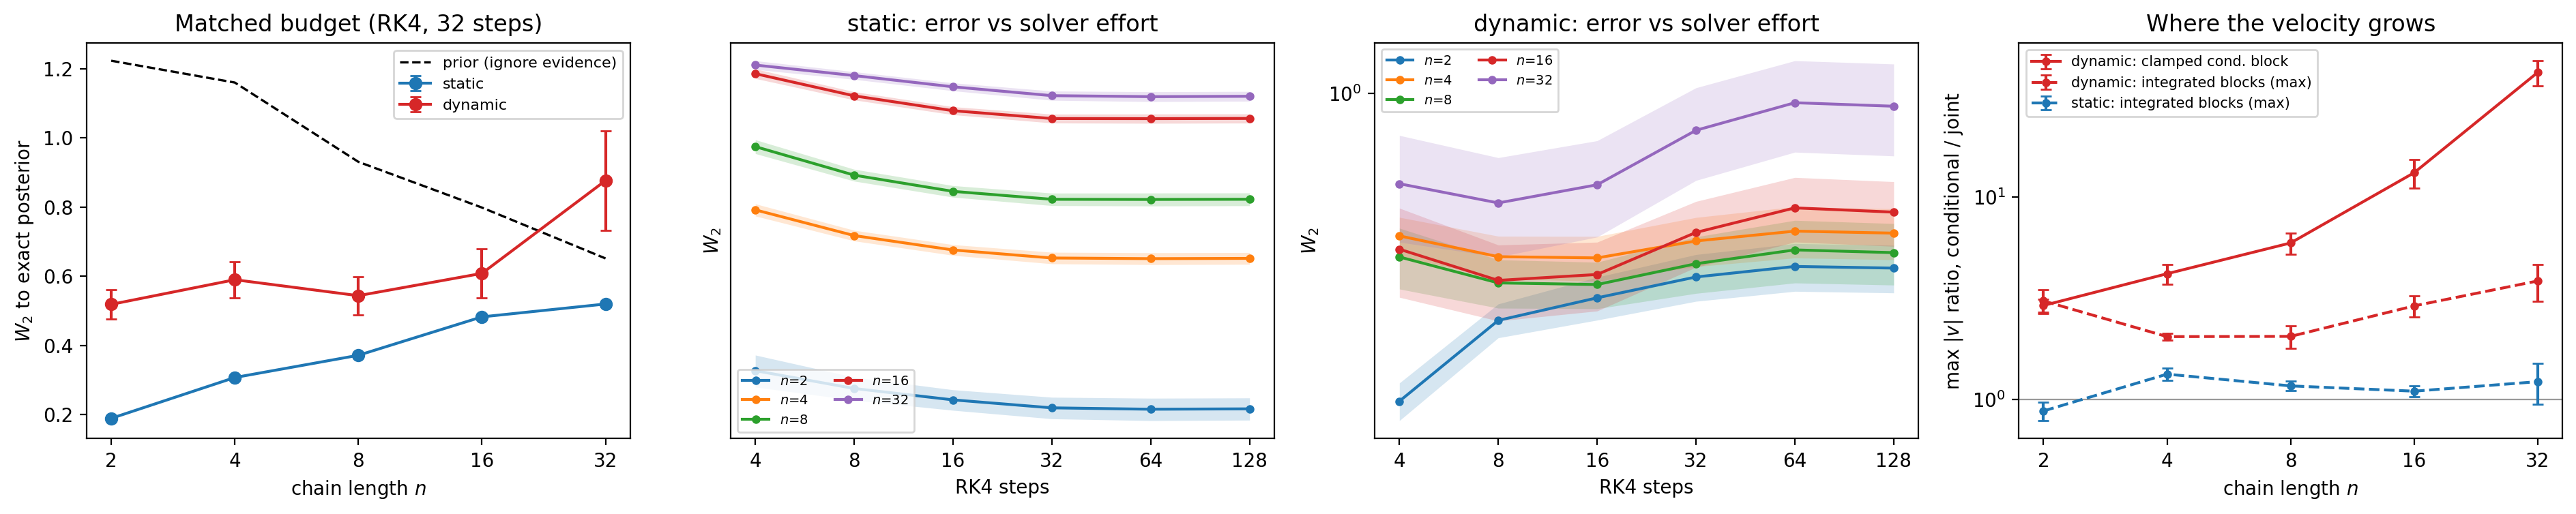
\includegraphics[width=0.93\textwidth]{images/ablations/chain_stiffness_rw.png}
    \caption{\textbf{Scaling dynamic conditioning on chains.} $W_2$ to the exact posterior of $p(x_0 \mid x_{n-1})$ on unit-root random-walk chains; $25$ evidence draws per depth, bands $\pm 1$ s.d.\ over $8$ seeds. \textbf{Far left:} matched budget ($32$ RK4 steps ${\approx}$ equal FLOPs): static grows slowly and monotonically; dynamic starts ${\sim}2.8\times$ worse, degrades with depth, and at $n{=}32$ crosses the dashed prior baseline (ignoring the evidence). \textbf{Middle:} static converges with step budget; dynamic \emph{anti-converges}. \textbf{Far right:} only the clamped condition block's velocity amplification grows with depth---the learned dynamics never stiffen.}
    \label{fig:chain-stiffness}
    \vspace{-0.8\baselineskip}
\end{figure*}